\documentclass{beamer}

%%%%%%%%%%%%%Solarized Theme%%%%%%%%%%%%%%%
\usecolortheme[dark,accent=cyan]{solarized}
\beamertemplatenavigationsymbolsempty

%%%%%Packages%%%%%
\usepackage{graphicx}
\usepackage{hyperref}
\usepackage{colortbl, xcolor}
\usepackage{booktabs}
\usepackage{standalone}
\usepackage{marvosym}
\usepackage{color}
\usepackage{animate,media9,movie15}

\usepackage{enumitem,amssymb}
\newlist{todolist}{itemize}{2}
\setlist[todolist]{label=$\square$}
\usepackage{pifont}
\newcommand{\cmark}{\ding{51}}%
\newcommand{\xmark}{\ding{55}}%
\newcommand{\done}{\rlap{$\square$}{\raisebox{2pt}{\large\hspace{1pt}\cmark}}%
\hspace{-2.5pt}}
\newcommand{\wontfix}{\rlap{$\square$}{\large\hspace{1pt}\xmark}}

\usepackage{tikz}
\usetikzlibrary{patterns}
\usetikzlibrary{calc}

\usepackage{minted}

\definecolor{DarkGray}{gray}{0.1}
\definecolor{DarkGray}{gray}{0.1}
\usemintedstyle{native}

\begin{document}

\begin{frame}
\centering
    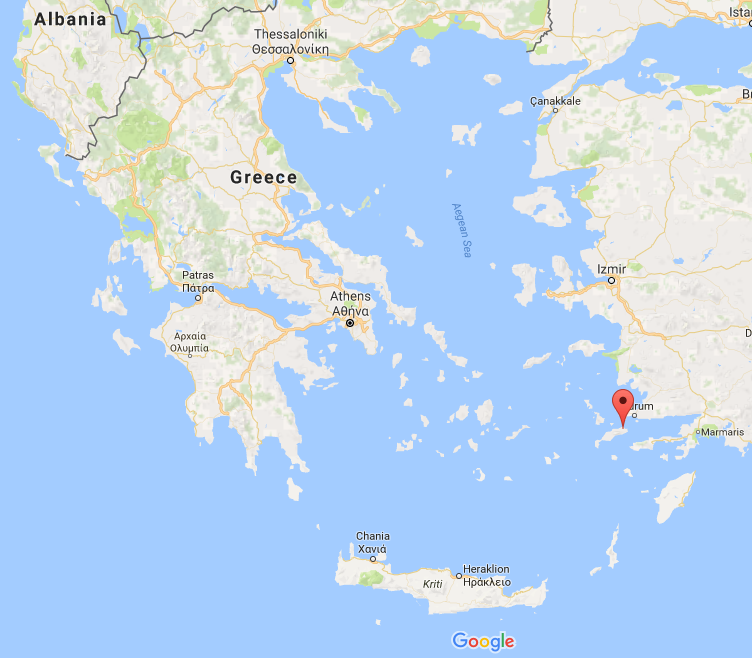
\includegraphics[width=.75\textwidth]{static/map-kos.png}
\end{frame}

\begin{frame}
    \begin{center}
    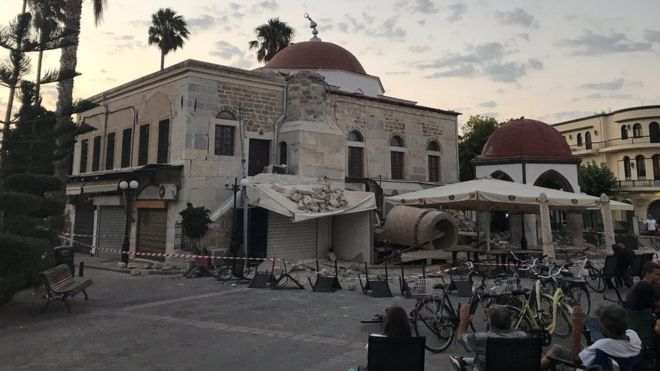
\includegraphics[width=0.65\textwidth]{static/earth_quake_kos.jpg}
    \vspace{10pt}
    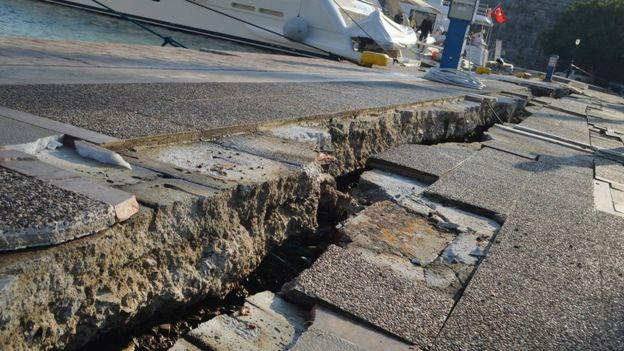
\includegraphics[width=0.65\textwidth]{static/quake_two.jpg}
    \end{center}
\end{frame}

\begin{frame}[fragile]
    \begin{minted}
    [
    framesep=4mm,
    baselinestretch=1.2,
    bgcolor=DarkGray,
    fontsize=\footnotesize
    ]
    {python}
>>> import quakefeeds
    \end{minted}

    \begin{minted}
    [
    framesep=4mm,
    baselinestretch=1.2,
    bgcolor=DarkGray,
    fontsize=\footnotesize,
    ]
    {python}
>>> from quakefeeds import QuakeFeed

>>> feed = QuakeFeed("2.5", "month")
>>> feed.title
'USGS Magnitude 2.5+ Earthquakes, Past Month'
    \end{minted}
\end{frame}

\begin{frame}[fragile]
    \begin{minted}
    [
    framesep=4mm,
    baselinestretch=1.2,
    bgcolor=DarkGray,
    fontsize=\tiny
    ]
    {python}
{'geometry': {'coordinates': [27.3346, 36.9405, 5.01], 'type': 'Point'},
 'id': 'us1000apsm',
 'properties': {'alert': None,
  'cdi': 4.1,
  'code': '1000apsm',
  'detail': 'https://earthquake.usgs.gov/earthquakes/feed/v1.0/detail/us1000apsm.geojson',
  'dmin': 0.962,
  'felt': 59,
  'gap': 45,
  'ids': ',us1000apsm,',
  'mag': 4.4,
  'magType': 'mb',
  'mmi': None,
  'net': 'us',
  'nst': None,
  'place': '6km NE of Kos, Greece',
  'rms': 0.82,
  'sig': 322,
  'sources': ',us,',
  'status': 'reviewed',
  'time': 1507665564350,
  'title': 'M 4.4 - 6km NE of Kos, Greece',
  'tsunami': 0,
  'type': 'earthquake',
  'types': ',dyfi,geoserve,origin,phase-data,',
  'tz': 120,
  'updated': 1508097562926,
  'url': 'https://earthquake.usgs.gov/earthquakes/eventpage/us1000apsm'},
 'type': 'Feature'}
    \end{minted}
\end{frame}

\begin{frame}
\centering
\Large{\textcolor{orange}{MATPLOTLIB BASEMAP TOOLKIT}}

\vfill 

\small{\url{http://introtopython.org/visualization_earthquakes.html}}  
\end{frame}


\begin{frame}[fragile]
\tiny{
\begin{columns}
\begin{column}{0.45\textwidth}
\begin{minted}
    [
    framesep=4mm,
    baselinestretch=1.2,
    bgcolor=DarkGray,
    fontsize=\tiny
    ]
{python}
from mpl_toolkits.basemap import Basemap
import matplotlib.pyplot as plt
import numpy as np

plt.figure()
my_map = Basemap(projection='ortho', 
                 lat_0=22,  lon_0=30.22, 
                 resolution='h')
my_map.drawcoastlines()








plt.show()
\end{minted}
\end{column}
\begin{column}{0.55\textwidth}
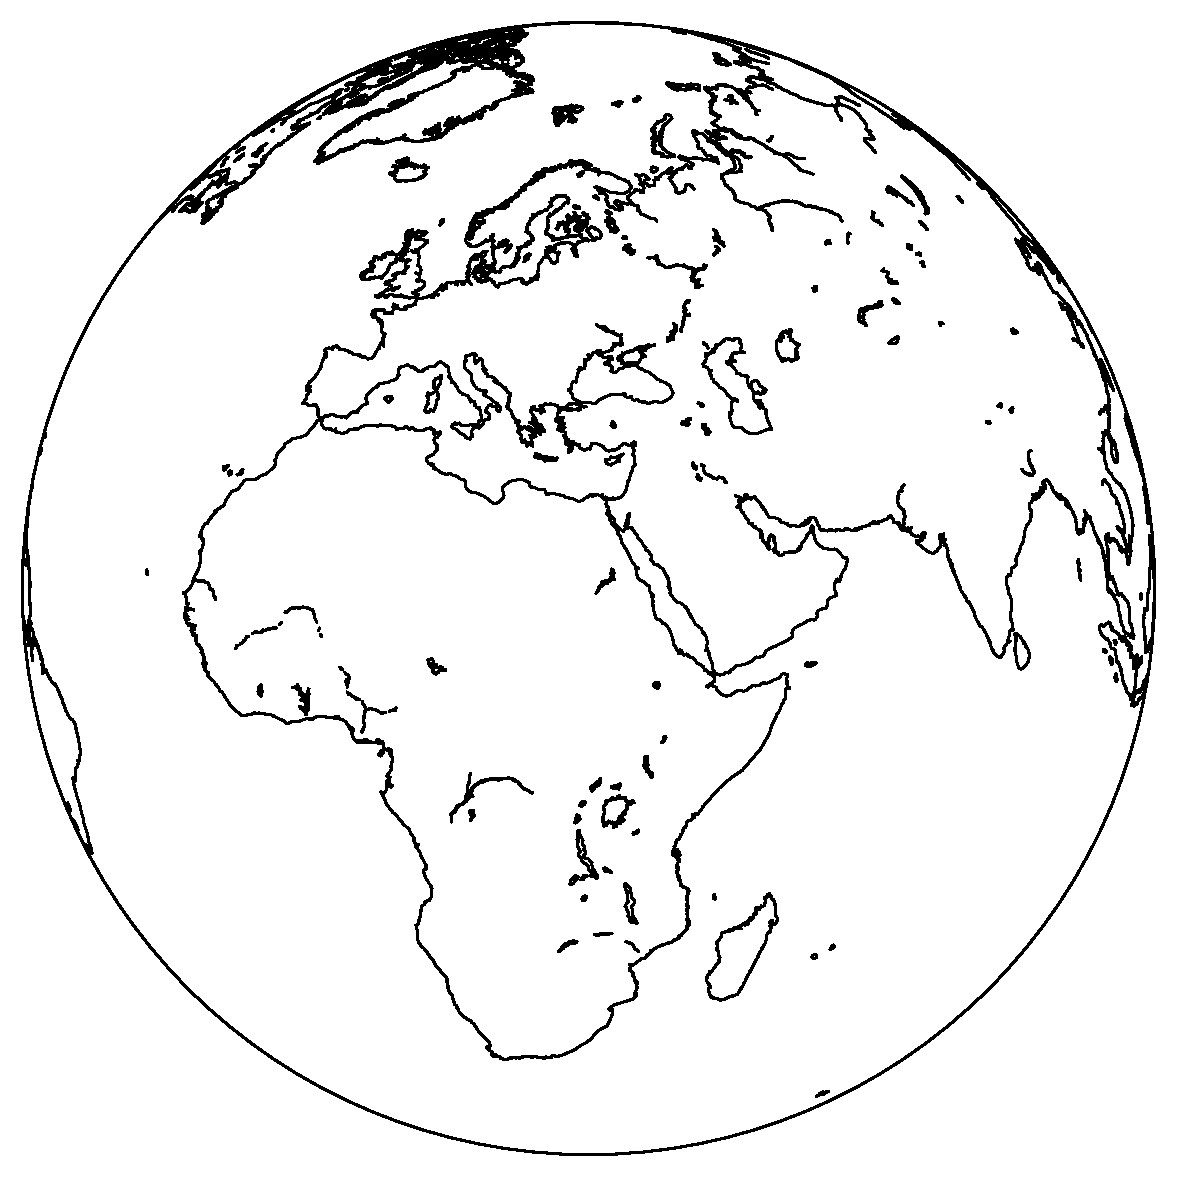
\includegraphics[width=\textwidth]{static/simple_map.pdf}
\end{column}
\end{columns}
}
\end{frame}

\begin{frame}[fragile]
\tiny{
\begin{columns}
\begin{column}{0.45\textwidth}
\begin{minted}
    [
    framesep=4mm,
    baselinestretch=1.2,
    bgcolor=DarkGray,
    fontsize=\tiny
    ]
{python}
from mpl_toolkits.basemap import Basemap
import matplotlib.pyplot as plt
import numpy as np

plt.figure()
my_map = Basemap(projection='ortho', 
                 lat_0=22,  lon_0=30.22, 
                 resolution='h')
my_map.drawcoastlines()
my_map.drawcountries()
my_map.fillcontinents(color='orange')
my_map.drawmapboundary()
 
meridians = np.arange(0, 360, 30)
parallels = np.arange(-90, 90, 30)
my_map.drawmeridians(meridians)
my_map.drawparallels(parallels)

plt.show()
\end{minted}
\end{column}
\begin{column}{0.55\textwidth}
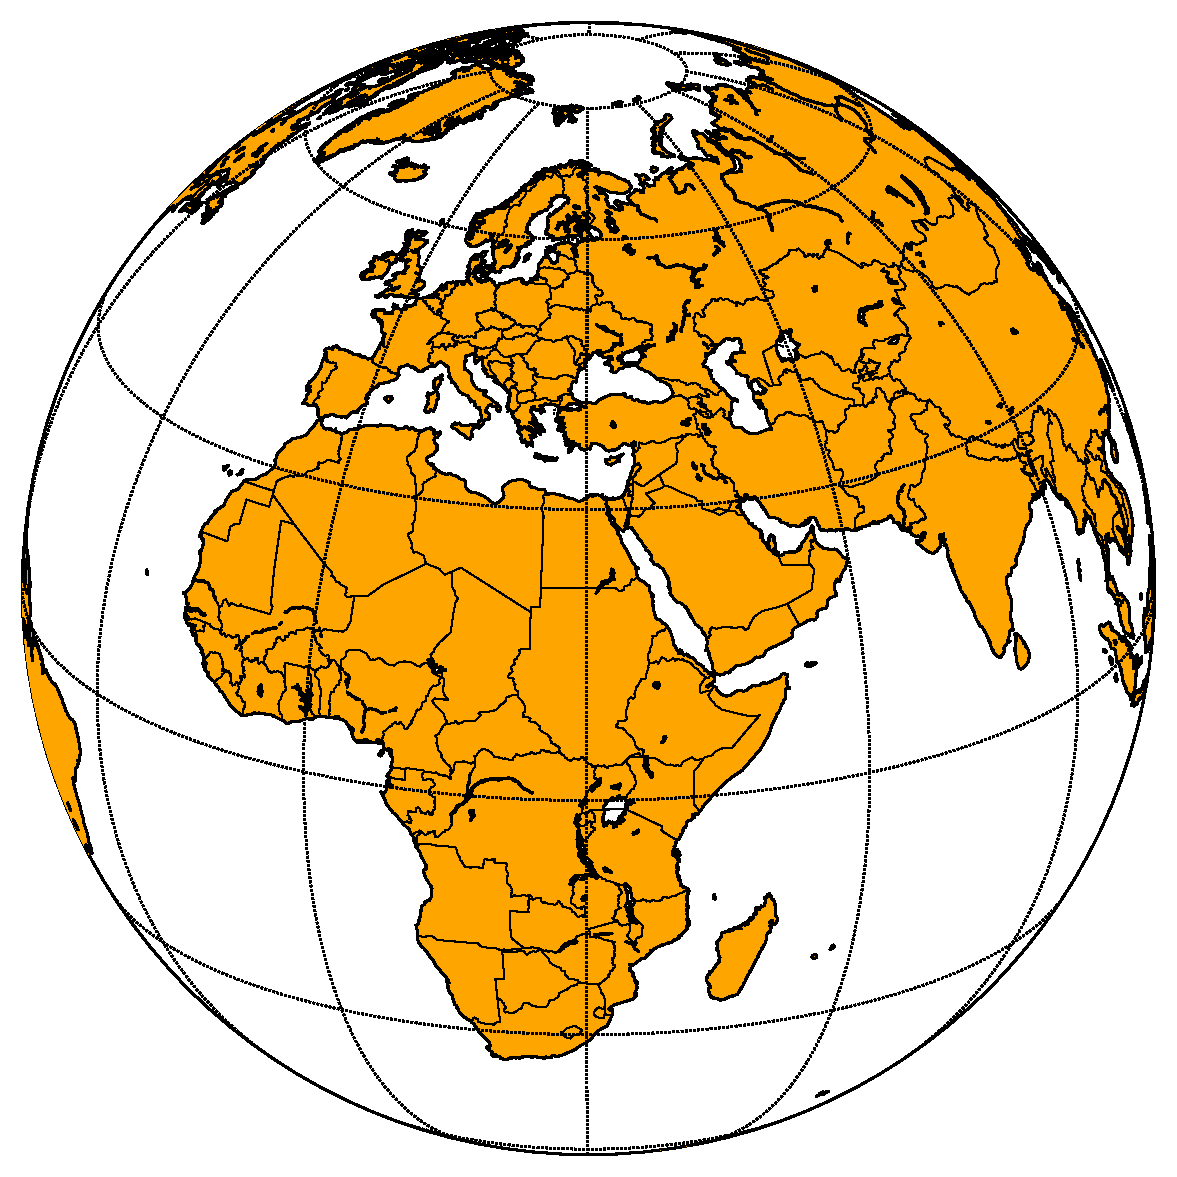
\includegraphics[width=\textwidth]{static/earth_map_two.pdf}
\end{column}
\end{columns}
}
\end{frame}

\begin{frame}
    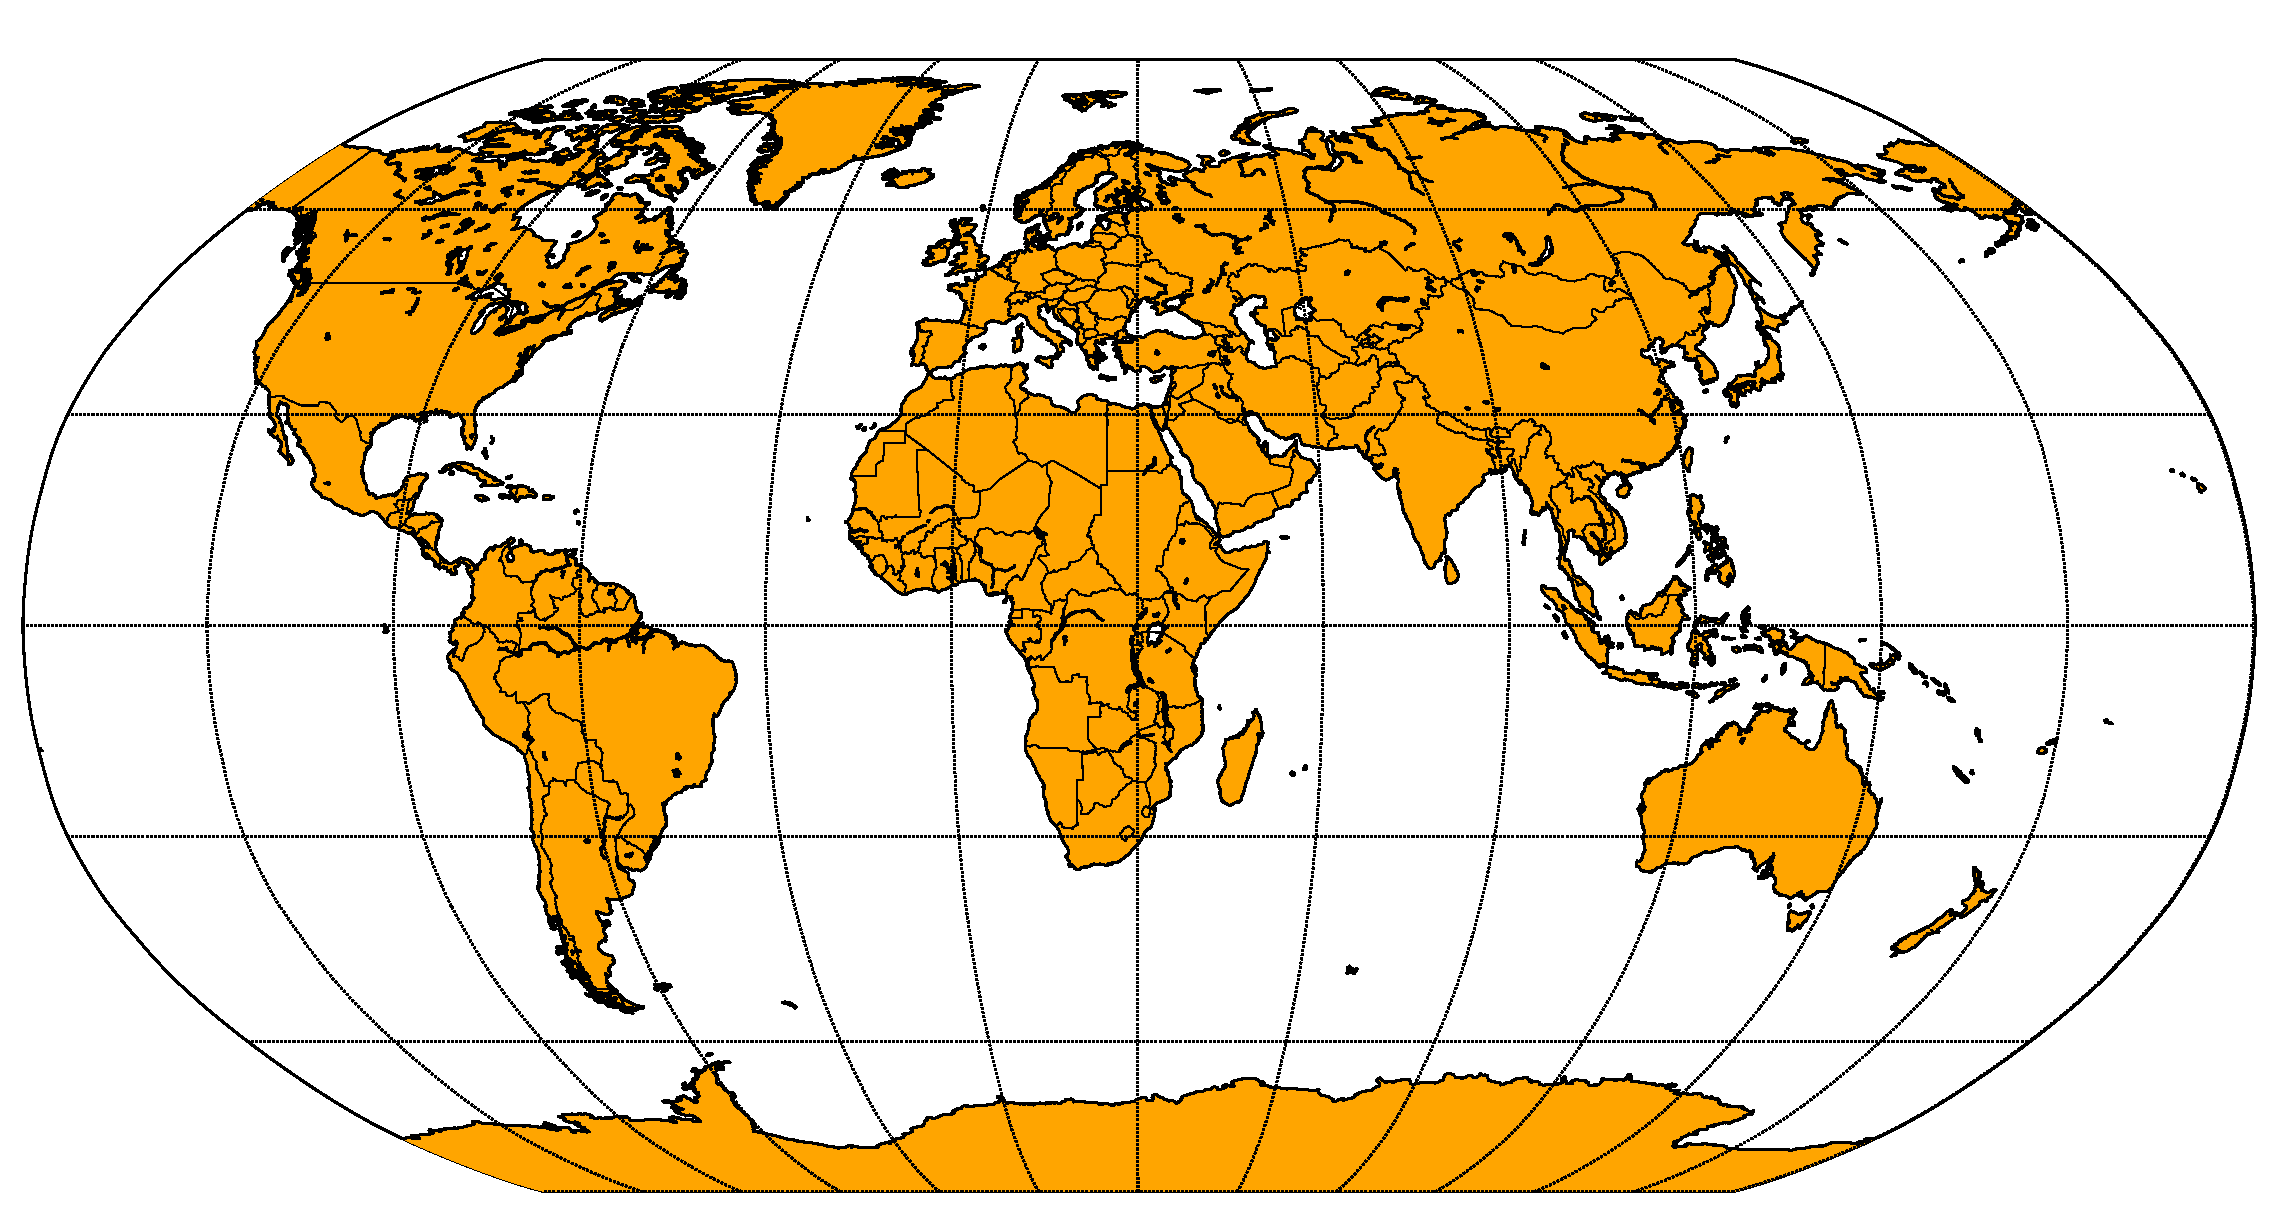
\includegraphics[width=1\textwidth]{static/part_2_map.pdf}
\end{frame}

\begin{frame}[fragile]
\tiny{
\begin{columns}
\begin{column}{0.45\textwidth}
\begin{minted}
    [
    framesep=4mm,
    baselinestretch=1.2,
    bgcolor=DarkGray,
    fontsize=\tiny
    ]
{python}
plt.figure()
my_map = Basemap(projection='merc', 
                 lat_0=40, lon_0=19,
                 resolution = 'h',
                 llcrnrlon=20.577,
                 llcrnrlat=33.568
                 urcrnrlon=28.1905, 
                 urcrnrlat=39.701)
 
my_map.drawcoastlines()
my_map.drawcountries()
my_map.fillcontinents(color='orange')




plt.axis('off')
plt.show()
\end{minted}
\end{column}
\begin{column}{0.51\textwidth}
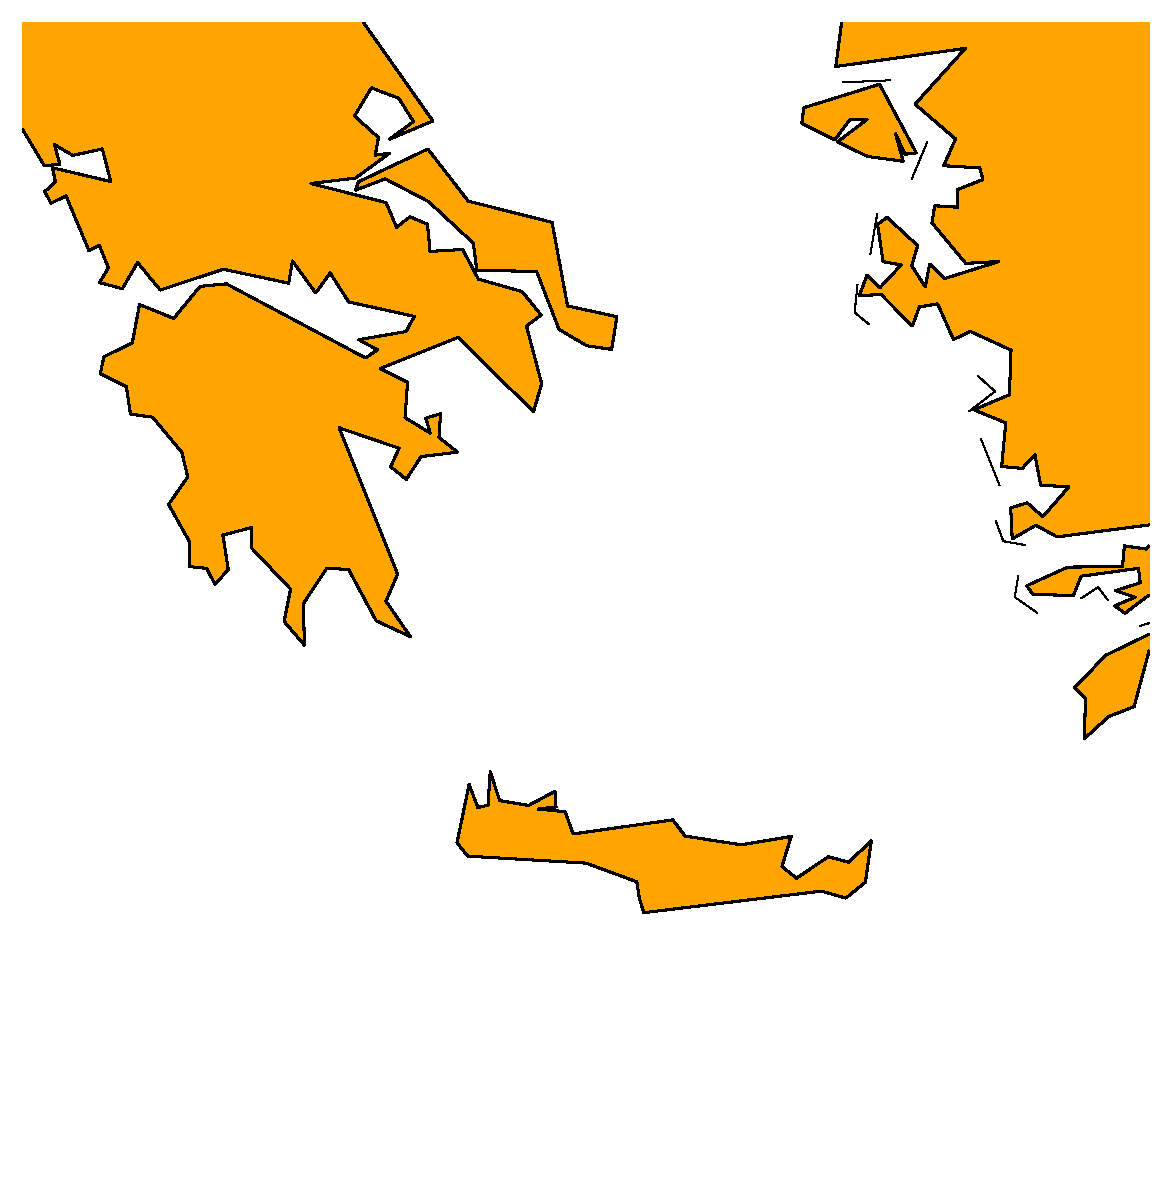
\includegraphics[width=\textwidth]{static/greece_map.pdf}
\end{column}
\end{columns}
}
\end{frame}

\begin{frame}[fragile]
\tiny{
\begin{columns}
\begin{column}{0.45\textwidth}
\begin{minted}
    [
    framesep=4mm,
    baselinestretch=1.2,
    bgcolor=DarkGray,
    fontsize=\tiny
    ]
{python}
plt.figure()
my_map = Basemap(projection='merc', 
                 lat_0=40, lon_0=19,
                 resolution = 'h',
                 llcrnrlon=20.577,
                 llcrnrlat=33.568
                 urcrnrlon=28.1905, 
                 urcrnrlat=39.701)
 
my_map.drawcoastlines()
my_map.drawcountries()
my_map.fillcontinents(color='orange')

x,y = my_map(lons, lats)
my_map.plot(x, y, 'ro', markersize=10)

plt.axis('off')
plt.show()
\end{minted}
\end{column}
\begin{column}{0.51\textwidth}
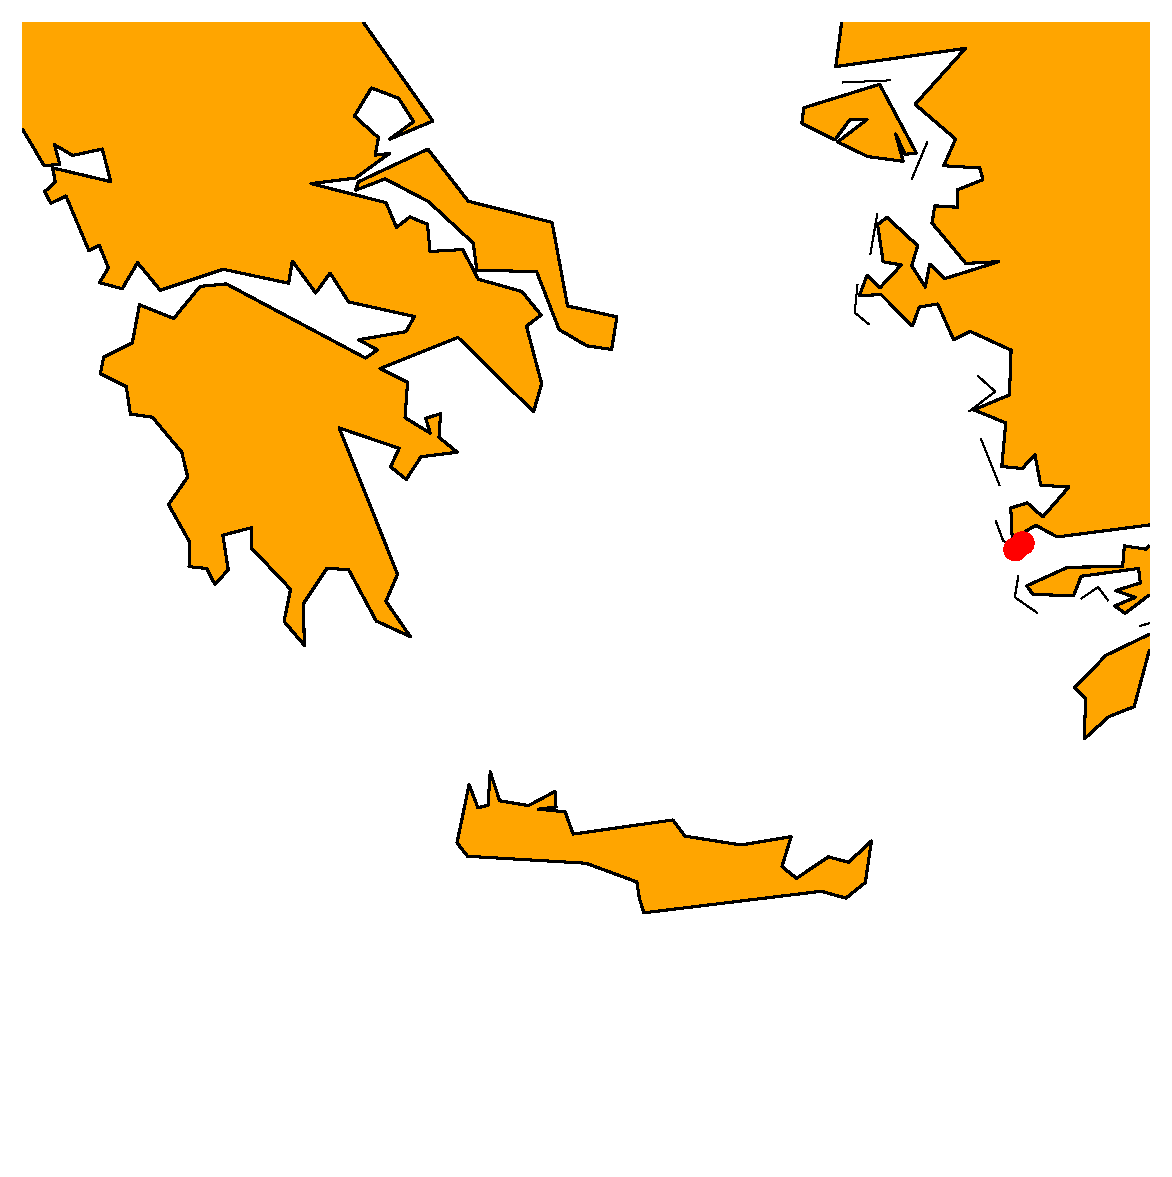
\includegraphics[width=\textwidth]{static/kos_map.pdf}
\end{column}
\end{columns}
}
\end{frame}

\begin{frame}
    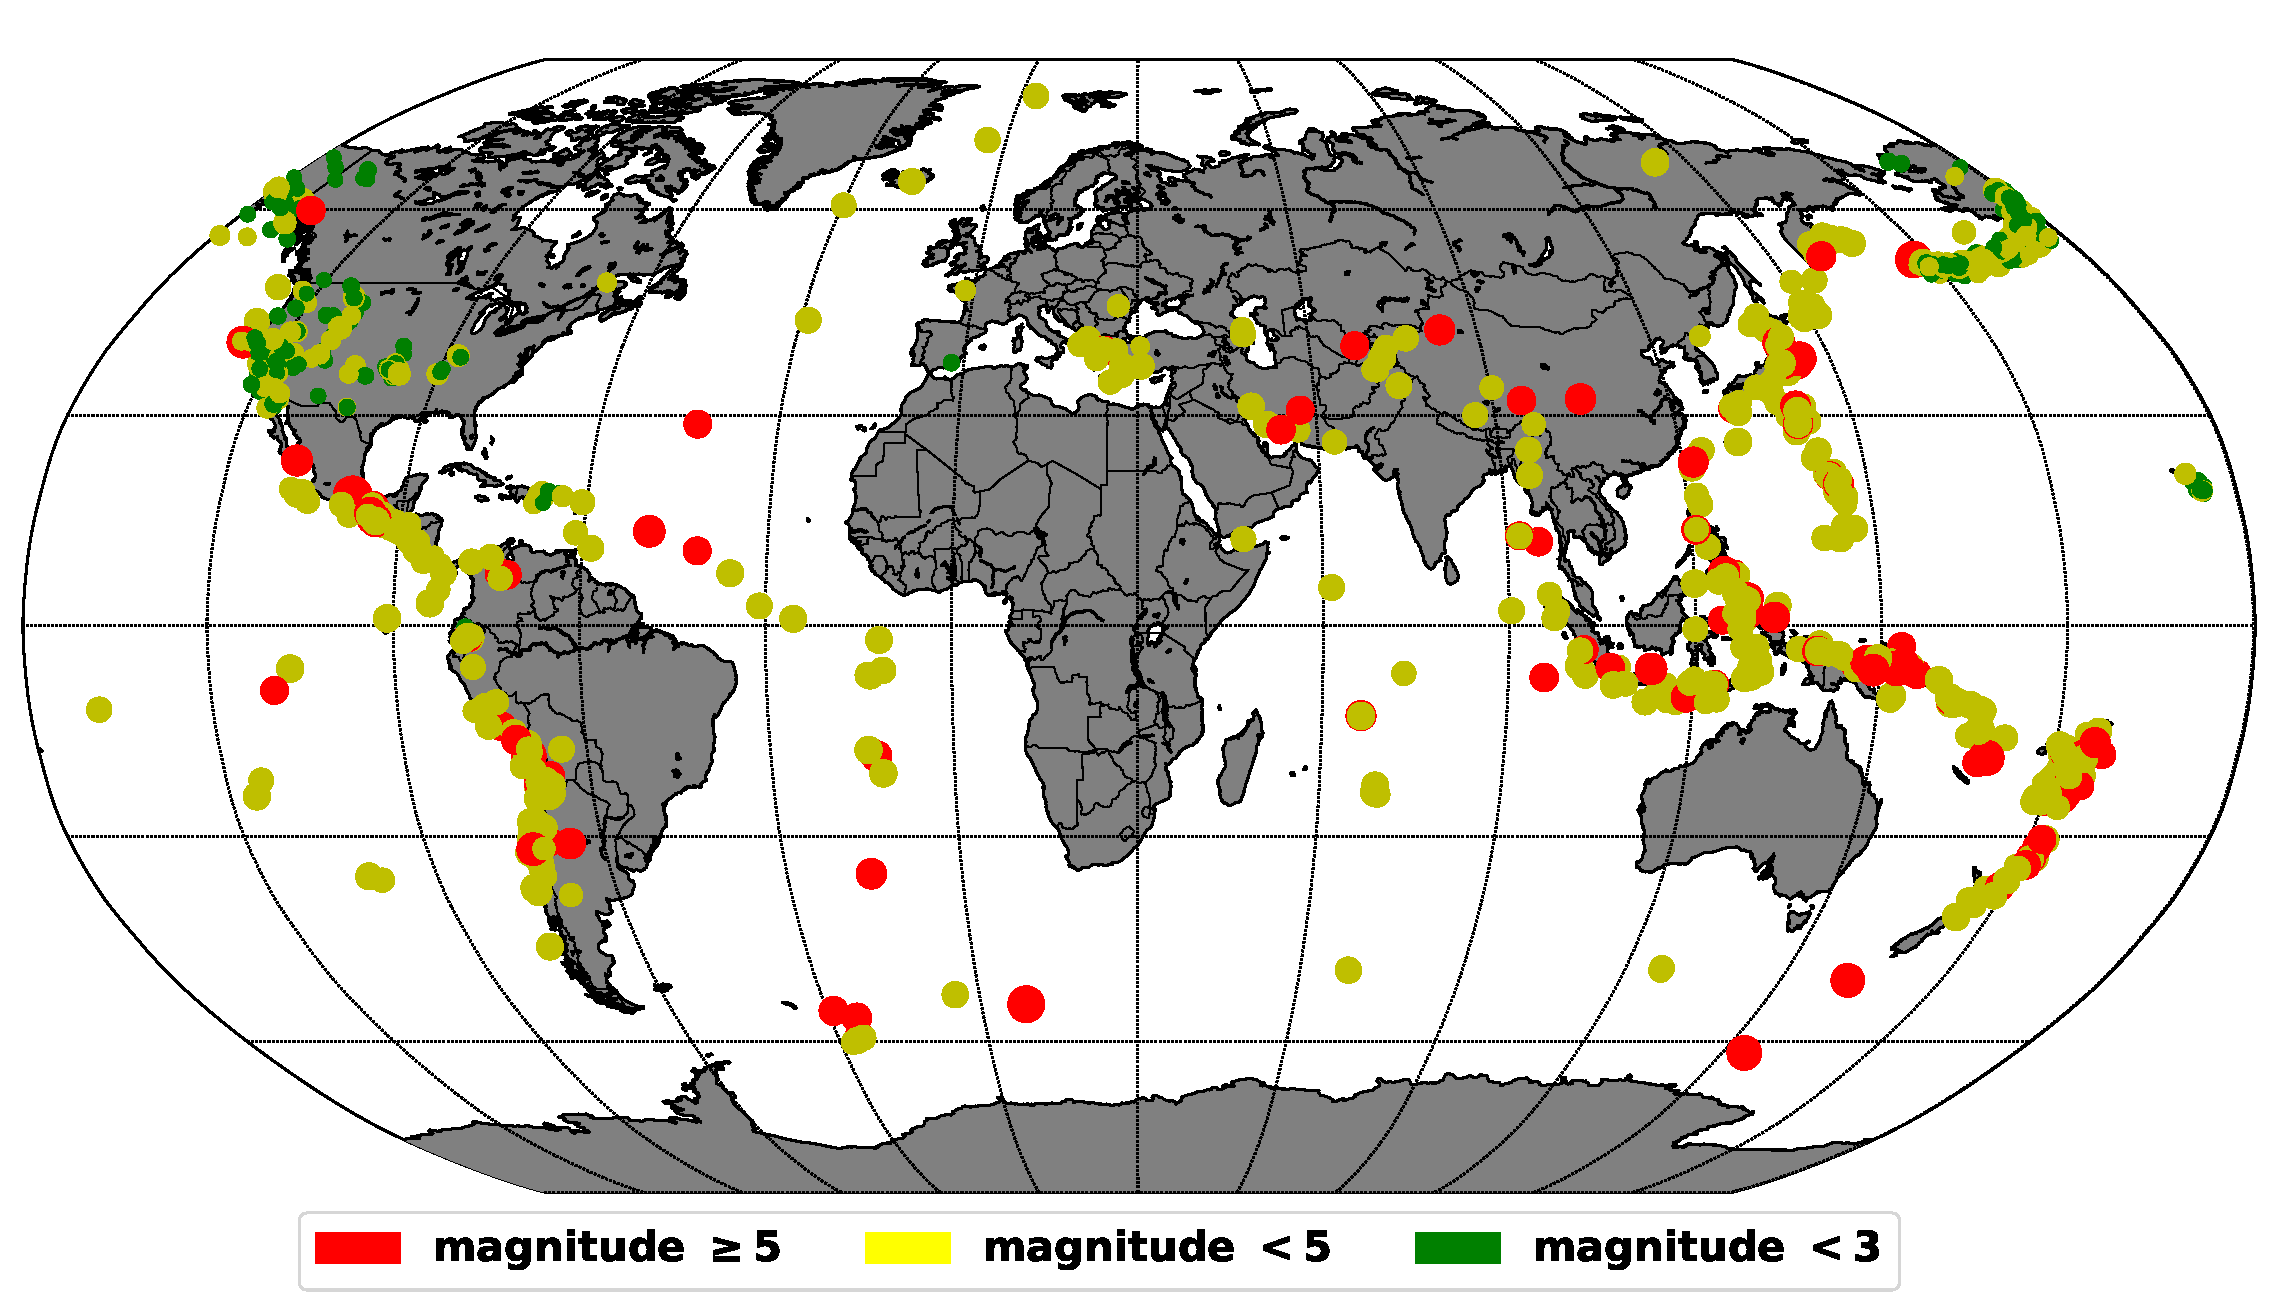
\includegraphics[width=\textwidth]{static/world_map.pdf}
\end{frame}

\begin{frame}[fragile]
	\begin{center}

\begin{minted}
    [
    framesep=4mm,
    baselinestretch=1.2,
    bgcolor=DarkGray,
    fontsize=\small
    ]
{python}
>>> import quakefeeds
\end{minted}

		\huge{\textbf{}}\\~\\
		\large{\url{http://introtopython.org/visualization_earthquakes.html}}\\
	\end{center}
\end{frame}

\end{document}

